\chapter{Introduction}
\label{chap:01}


\paragraph{}
The vibration phenomenon can be observed in various standard settings, including speaking, vision, auditioning, and other activities involving human interaction owing to mechanical waves and digital communication via electromagnetic waves \cite{tse1963mechanical}. Also, Vibrations are a part of our everyday lives, and individuals encounter them in various ways. This phenomenon is required in various engineering applications, such as car suspension, where vibration increases driver comfort. They range from small-scale motions of atoms in substances to large-scale swaying of buildings and other structures and can be welcomed and intended, or bothersome and, in the worst case, harmful \cite{mori2017mechanical}. Oscillatory motion is joint, and physicists frequently idealise these examples of vibration into instances of a beneficial fiction, the harmonic oscillator. 

A mathematical depiction of a physical, biological, or information system is a simulation \cite{wada1972equivalent}. Models enable us to think about a system and forecast its behaviour. A dynamical system is one in which the consequences of actions do not arise instantly. For example, a headache does not go away immediately after taking aspirin; it takes time to take action. Additional funding for a development project does not enhance profits in the short term, but it may do the same in the longer - term in enterprise applications. All of these are instances of dynamical systems, in which the system's behaviour varies through time. As previously stated, the mass-spring model has been widely utilised to simulate deformable objects for facial animation \cite{keeve1998deformable}, animation of artificial animals \cite{tu1994artificial}, cloth draping \cite{ji2006three}, garment animation \cite{provot1995deformation}, and, more recently, surgical simulations \cite{sorensen2007virtual}. Recent enhancements to this model include the inverse dynamics approach to eliminate super elongation of the springs \cite{mozafary2016study} and the implicit integration method to take substantial time steps. 


The mass-spring model can be considered a discrete approximation method for solving the Lagrange partial differential equation of motion \cite{baleanu2020new}. Because of the extreme discretisation, the mass-spring model will only approximate the continuous object in some ways. The mass-spring model and the finite element method (FEM) \cite{duan2014volume} were compared, and it was determined that an exact simulation using the mass-spring model is unattainable. This project could clarify why there hasn't been much research on optimising the parameters of the mass-spring model. Even though the mass-spring model cannot provide an exact simulation, certain reasonable parameter sets provide more physically realistic simulations than others. The mass-spring model is currently implemented using a trial-and-error approach to determine parameter values for many applications. Aside from the fact that the criteria are highly subjective, the process is extremely laborious and time-consuming.

The capacity to forecast and reduce structural vibrations has recently attracted more attention. Vibrations originate from either external sources, such as wind, or internal sources, including friction between mechanical pieces of a system. The most typical scenario of vibration is break squeal in automobiles \cite{suggs1969application}. As a result, researchers have focused their efforts on studying vibration phenomena and their applicability in real life \cite{levitan1960forced} \cite{pellicer2004analysis} \cite{grandmont2006viscoelastic}. Because their occurrence is inherently dependent on the unique internal properties, the motion can be described mathematically as the unstable homogeneous solution to the homogeneous equations of motion. Furthermore, mathematical solutions will be discussed in detail in future chapters. 

\section{Background of the study}
\label{sec:1.1}

\paragraph{}

The study of linked oscillators has since become an important branch of mathematics, with applications in physics, biology, and chemistry \cite{Chapter427:online}. Coupled oscillators are seen in biological systems as well \cite{winfree1967biological} \cite{hannay2018macroscopic}. Most species directly correspond to numerous patterns in our environment, such as the earth's rotation around the sun, the alternation of night and day, or the tides. Organisms demonstrate periodicities due to their environment and exhibit innate periodic activity. Inhalation, blood circulation, chewing, molecular motion and galloping are all instances of rhythmic motion patterns. Waves are the propagation of oscillations in space caused by the connection of individual oscillators. A straightforward exercise is to strike the right piano note, which sounds the tuning-fork tuned to the same frequency as the key we hit. Another scenario is the powerful sound of the frequency corresponding to the resonance frequency of the glass breaking a delicate wine glass. In this section coupled oscillators, Degree of freedom, Euler's Lagrange, Runge kutta method (fourth order) and other relevant background will be discussed. 


\subsection{Coupled oscillators}

\paragraph{}

Like the small-amplitude swinging of a pendulum, some oscillations are extremely simple and can be approximated by a single mass on the end of a Hooke'slaw spring. And some are more complex but could still be represented by two or more masses and two or more springs. Examples are compound mechanical systems, oscillating electrical circuits with multiple branches, multi-atom molecules, and elastic materials.  Here we display the few example of coupled oscillators used to understand oscillations like these.

\subsubsection{Linear systems of masses and springs}
As shown in Figure \ref{fig:1}, the blocks are attached to three springs, and the outer springs are likewise attached to stationary walls. The outer springs each have a force constant $k$, while the inner spring has a force constant $k'$. When the blocks are at rest, the springs are untethered. Let $x_1$ and $x_2$ represent the displacements of blocks 1 and 2 from their equilibrium locations, positive to the right. Assume three blocks are connected to four springs: In the equilibrium position, the springs are again unstretched, and the blocks can only move horizontally. Each outer spring's far end is linked to a stationary wall. The three blocks' displacements from equilibrium are $x_1$,$x_2$, and $x_3$, all positive to the right. Assume the blocks have the same mass $m$ and the same force constant $k$, as shown in Figure \ref{fig:5}.


 \begin{figure}[hbt!]
	\centering
	\begin{framed}
	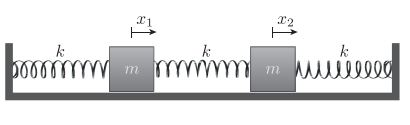
\includegraphics[width=0.6\textwidth]{Figures/A.JPG}
	\end{framed}
	\caption{Two blocks are attached to three springs \cite{Departme83:online}.}
	\label{fig:1}
\end{figure}

 \begin{figure}[hbt!]
	\centering
	\begin{framed}
	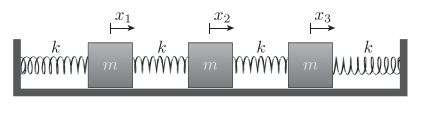
\includegraphics[width=0.6\textwidth]{Figures/E.JPG}
	\end{framed}
	\caption{Three blocks are attached to four springs \cite{Departme83:online}.}
	\label{fig:5}
\end{figure}

So far, we've only worked with masses attached to Hooke's law springs, which are, of course, highly idealised systems. More realistically, for macroscopic one dimensional mechanical motions here we concerned $CO_2$ molecules. As illustrated in Figure \ref{fig:4}, carbon dioxide is a linear molecule with the carbon atom (of mass m and coordinate x2) in the middle and the oxygen atoms (of mass M and coordinates x1 and x3) at the two ends. The behavior of the atoms at the scale of molecules is, of course, governed by quantum mechanics, and hence classical mechanics is merely a rough approximation to the true behaviour of the $CO_2$ molecule.

 \begin{figure}[hbt!]
	\centering
	\begin{framed}
	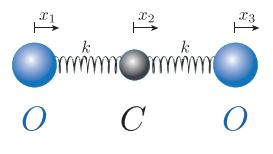
\includegraphics[width=0.35\textwidth]{Figures/D.JPG}
		\end{framed}
	\caption{The carbon dioxide molecule \cite{Departme83:online}.}
	\label{fig:4}
\end{figure}

\subsubsection{Coupled pendulums}

Two m-mass balls are tied to two equal-length $l$ strings to form side-by-side pendulums of equal period. As shown in Figure \ref{fig:2}, a weak spring $k$ is now coupled to the two balls. 

 \begin{figure}[hbt!]
	\centering
	\begin{framed}
	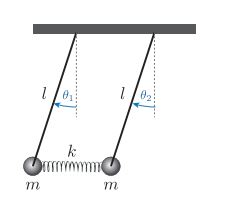
\includegraphics[width=0.38\textwidth]{Figures/B.JPG}
		\end{framed}
	\caption{Coupled pendulum \cite{Departme83:online}.}
	\label{fig:2}
\end{figure}

\subsubsection{ A planar system: masses in an equilateral triangle}

All particles and springs were aligned along a straight line and were only permitted to oscillate along that same straight line. Figure \ref{fig:3} depicts the normal-mode oscillations of a system with three equal masses $m$ and three equal springs $k$ in the shape of an equilateral triangle.

 \begin{figure}[hbt!]
	\centering
	\begin{framed}
	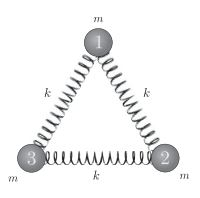
\includegraphics[width=0.33\textwidth]{Figures/C.JPG}
	\end{framed}
	\caption{Masses in an equilateral triangle
 \cite{Departme83:online}.}
	\label{fig:3}
\end{figure}

When a system is aroused into oscillations that are a mixture of normal modes \cite{cochelin20197th}, the motion will alter with time. Perhaps one of the masses will decrease amplitude and transfer energy to another mass, which will then return the energy \cite{kerschen2009nonlinear}. Even if the oscillations are all at the same frequency, such motion is totally distinguishable from simple harmonic motion and hence does not represent a normal mode. The transfer of energy usually occurs at a frequency that is significantly different from the frequency of oscillation.

\subsection{Degree of freedom}

\paragraph{}

Assume there are $N$ particles that can only move in one dimension. Then we define there seem to be N degrees of freedom (DOF) \cite{rosenberg1962normal}, $x_1, x_2,...x_N$, which are the positions observed along each particle's single dimension. If somehow the $N$ particles are instead permitted to travel in two dimensions, there are $2N$ degrees of freedom (DOF), $x_1, y_1,...x_N, y_N$, and so on. In case of that, Degrees of freedom (DOF) relate to the maximum number of logically independent values in a data sample, which are values with the freedom to fluctuate. DOF can be calculated using the below equation \eqref{1} and its corresponding constant values. 

\begin{equation}
    \label{1}
    DOF = (N \times n ) - k
\end{equation}

Where, \\
$n$ =  Number of dimensions \\
$N$ = Number of particles\\
$k$ = Number of constraints


\subsection{Euler-Lagrange equation}
\label{lag}

\paragraph{}

In this section, we'll learn about an entirely new way of seeing the world. Imagine the mass on the end of a spring. Of course, we can evaluate this by using $F = ma$ (Newton's second law) \cite{sharma2014isaac} to write out $m\Ddot{x} = k\Dot{x}$ \cite{zhong2019reliability}. As we all know, the solutions to such an equation are sinusoidal functions. However, we can sort things out by utilising a different strategy that does not reinforce F = ma. This new strategy is preferable to using Newton's second law in many (perhaps most) physical conditions. Here we now look at the lagrangian method. 

\begin{equation}
    \label{2}
    F_i = m\Ddot{x_i}
\end{equation}

The kinetic energy function, which is the time derivative of the momentum $p_1 = \partial T / \partial \Dot{x}$, determines the right side of this equation \eqref{2}. while the right hand side is a derivative of the potential energy, $- \partial U / \partial x_i$. . As $T$ is independent of $x_i$ and $U$ is independent of ˙$x_i$ in these coordinates, In terms of the Lagrangian, we can write both sides. 

\begin{equation}
    \label{3}
    L = T -U 
\end{equation}

Which is then a function of both the coordinates and their velocities. Thus we have established which will be known as Lagrange’s equation

\begin{equation}
    \label{4}
    \frac{d}{dt}(\frac{\partial L}{\partial \dot{xi}})-\frac{\partial L}{\partial xi} = 0 
\end{equation}

Here, $x = (x_1, . . . , x_N )$ and likewise $\dot{x}˙ = (\dot{x_1}, . . . , \dot{x_N})$. And also we can write \eqref{3} where
$T$ is the kinetic energy and $V$ is the potential energy. In the simplest cases, $T = T(\dot{x})$ and $V = V (x)$, The solution to a given mechanical problem is obtained by solving a set of $N$ second-order differential equations known as Euler-Lagrange equations of motion,

\begin{equation}
    \label{5}
    \frac{d}{dt}(\frac{\partial L}{\partial \dot{xi}})-\frac{\partial L}{\partial xi} = 0 
\end{equation}

\subsection{Numerical analysis}
\label{Num}

\paragraph{}
Numerical analysis is a branch of mathematics that teaches computer methods for studying and solving mathematical issues \cite{burden2015numerical}. In this section, we look at numerical approaches for solving the most frequent mathematical problems and analyse the errors that can occur while using these methods. Because practically all computation is now done on digital computers, we also explore the consequences for numerical method implementation.

The investigation of error is vital to numerical analysis. Most numerical approaches produce responses that are simply approximations to the intended genuine solution, and it is critical to understand the associated error and, if feasible, estimate or constrain it \cite{heydari2016theoretical}. This study looks at the numerous errors that can occur in a situation. The representation of numbers in computers, as well as the mistake in computer arithmetic, are investigated \cite{cui2018numerical}. The general results on the propagation of errors in calculations are presented, along with a detailed examination of errors in summing processes. Especially in this study, we will consider the Runge Kutta fourth-order (RK4) method \cite{islam2015accurate}. 

\subsubsection{Runge Kutta fourth order method}
\label{RK}
The fourth-order Runge-Kutta technique explains the lengthy computation of numerous unknowns, and the comprehensive step-by-step derivation and analysis can be found in many publications \cite{tan2012general} \cite{mehdi2017using}. Because of the method's importance in mathematics and applied science/engineering. By reviewing specific, possibly well-known papers, we simplify and minimise the complexity of their derivation and analysis by proposing a step-by-step derivation of the method.

In 1901, two German men, Carl Runge (1856-1927) and Martin Kutta (1867-1944), devised the Runge-Kutta Method \cite{tobies2012iris}. Carl Runge created numerical methods for solving the differential equations that evolved from his research on atomic spectra. These numerical techniques are still in use today. He employed so much mathematics in his studies that physicists mistook him for a mathematician, and he employed so much physics that mathematicians mistook him for a physicist. His name is now synonymous with the Runge-Kutta methods for numerically solving differential equations. Kutta, another German applied mathematician, is well recognised for his contribution to the Kutta-Joukowski theory of airfoil lift in aerodynamics, which is based on differential equations \cite{trefethen2015invented}. 

\newpage

\subsubsection{Runge-Kutta 4th order method to solve differential equation}

Given following inputs \cite{RungeKut7:online}. 

\begin{itemize}
    \item An ordinary differential equation that expresses the value of $dy/dt$ in terms of $t$ and $y$.
    \item Initial value of $y$, i.e., $y(0)$. 
\end{itemize}

\begin{equation}
    {{dy(t)} \over {dt}} = y'(t) = f(y(t),t), \quad \quad {\rm{with\;}} y(t_0)=y_0
\end{equation}

The evolution of the Fourth Order Runge-Kutta method closely parallels that of the second Order and will not be discussed in depth here. The fourth order method, like the second order method, has several variations that all employ four estimates to the slope. To determine the slope at some time t0 (assuming we just have an approximation to $y(t_0)$ (which we call $y^*(t_0)$), we will utilise the following slope approximations.

 \begin{figure}[hbt!]
	\centering
	\begin{framed}
	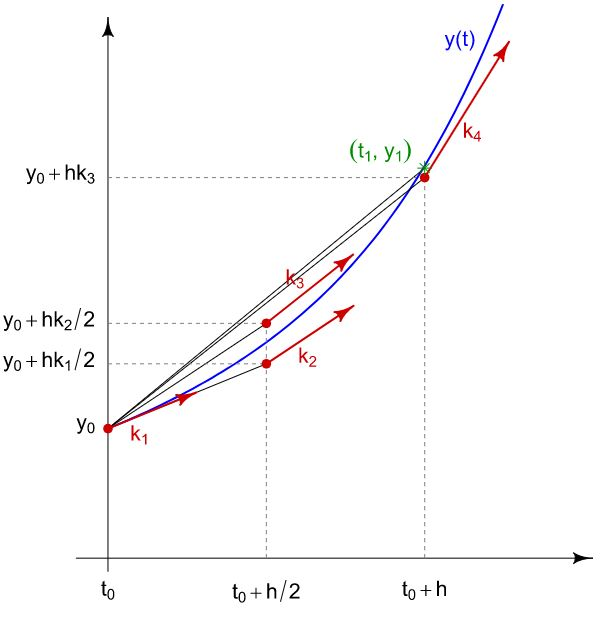
\includegraphics[width=0.6\textwidth]{Figures/F.JPG}
		\end{framed}
	\caption{Slopes used by the classical Runge-Kutta method \cite{hossain2017comparative}.}
	\label{fig:6}
\end{figure}

\newpage

\begin{equation}
    {k_1} = f({y^*}({t_0}),{t_0})
\end{equation}

\begin{equation}
    {k_2} = f\left( {{y^*}({t_0}) + {k_1}{h \over 2},{t_0} + {h \over 2}} \right)
\end{equation}

\begin{equation}
     {k_3} = f\left( {{y^*}({t_0}) + {k_2}{h \over 2},{t_0} + {h \over 2}} \right) 
\end{equation}

\begin{equation}
    {k_4} = f\left( {{y^*}({t_0}) + {k_3}h,{t_0} + h} \right)
\end{equation}

Each one of these slope estimates can be directly explained \cite{FourthOr20:online}.

\begin{itemize}
    \item $k_1$ is the slope at the beginning of the time step (this is the same as $k_1$ in the first and second order methods).
    
\item If we use the slope $k_1$ to step halfway through the time step, then $k_2$ is an estimate of the slope at the midpoint. This is the same as the slope$_2$, from the second order midpoint method. This slope proved to be more accurate than $k_1$ for making new approximations for y(t).

\item If we use the slope $k_2$ to step halfway through the time step, then $k_3$ is another estimate of the slope at the midpoint.

\item Finally, we use the slope, $k_3$, to step all the way across the time step$(t_0, t_0+h)$, and $k_4$ is an estimate of the slope at the endpoint. 
\end{itemize}

We then use a weighted sum of these slopes to get our final estimate of $y^*(t_0+h)$.

\begin{equation}
    {y^*}({t_0} + h) = {y^*}({t_0}) + {{{k_1} + 2{k_2} + 2{k_3} + {k_4}} \over 6}h 
\end{equation}



\begin{equation}
   {y^*}({t_0} + h) = {y^*}({t_0}) + \left( {{1 \over 6}{k_1} + {1 \over 3}{k_2} + {1 \over 3}{k_3} + {1 \over 6}{k_4}} \right)h
\end{equation}

\begin{equation}
   {y^*}({t_0} + h) =  {y^*}({t_0}) + mh
\end{equation}

 {\rm{where\;}}m{\rm{\;is\;a\;weighted\;average\; slope\; approximation.}}

The approach is comparable to the second order endpoint method \cite{dontchev2000second}, which employed an equal weighting of the slopes at the start and end of the interval. The weighting of the midpoint slopes ($k_2$ and $k_3$) is larger than that of the endpoint slopes ($k_1$ and $k_4$) in this case, because we expect these to be a better estimate of the slope while travelling from $y^*(t_0)$ to $y^*(t_0+h)$.


\newpage
\section{Problem statement and objectives}
\paragraph{}
Vibration analysis for frequency response and temporal response has become essential for significant industrial machines and other troubleshooting applications. The computation of natural frequencies for a finite coupled freedom system (one dimension and two dimension)  n-degree freedom system (one dimension and two dimension) and comparative amplitudes of vibrating masses assists the designer in selecting system parameters and allow the implementation for safer operations. As we all know, classical mathematical approaches are insufficient for real-time frequency response processing because they require more time and effort. We sought to examine a few freedom system for natural frequencies and hence pure mode forms in this study. The pure mode patterns can then be placed to obtain the system's real displacement pattern. We created below coupled freedom system by writing a software in the MatLab platform. The project objectives proposed for this study are expected to contribute to the current level of knowledge regarding the dynamic behaviour of coupled spring-mass systems compared to numerical solutions. The objectives
are listed below.

\begin{enumerate}
    \item Investigate the motion for undamped linear systems with  coupled two degrees of freedom.
    \item Investigate the motion for undamped linear systems with coupled many degrees of freedom. 
    \item Investigate the two-dimensional spring motion: the mass
m is free to move in the $XY$ plane. 
\end{enumerate}




\section{Project structure}
\paragraph{}

In the chapter one, introduction into the project and other background of study will be discussed. This chapter is presented coupled oscillations, degree of freedom, Lagrangian and numerical methods. In this chapter problem scope of the project and objectives will be discussed as well.  When it comes to the chapter two, there will be discussed the process and concepts corresponding to the methodology. Behalf of the methodology, above mentioned objectives will be explained under each and each sections. Both 1D and 2D spring mass models are considered their behaviour, assumptions and behind scene of the physics background. This will be demonstrated the both physics and mathematical concepts to explain the given objectives.  After that, in the chapter three,  the before obtaining the results theoretically  all obtained differential equations will be solved and explained by numerical method of Runge kutta fourth order. In chapter four, all the results of spring mass models will be discussed. Finally, chapter six brings the conclusion of the whole project.   
\paragraph{}






































